\subsubsection{Synthesis of homoserine lactone-ciprofloxacin triazole conjugates with cleavable linkers\label{sec:cleavable}}

In addition to the conjugates shown in the previous section, a further collection was synthesised in collaboration with Prof. Eddy Sotelo, a visiting researcher in the Spring group. Prof. Sotelo synthesised two alkyne-linked ciprofloxacin derivatives \compound{cmpd:Y4HCip} and \compound{cmpd:Y4MeCip} (see \ref{fig:cleavable_Ys}), both with cleavable linkers (see \ref{sec:intro})\todo{link this up}. 

\begin{figure}[H]
	\begin{center}
		\schemeref[Y4HCip]{cmpd:Y4HCip}
		\schemeref[Y4MeCip]{cmpd:Y4MeCip}
		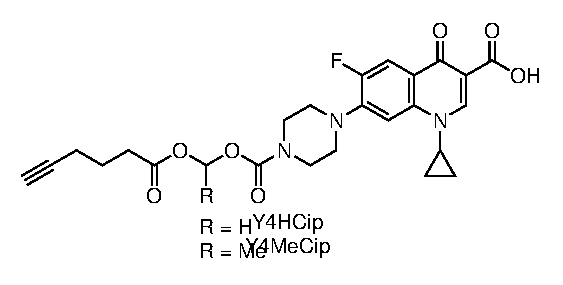
\includegraphics[scale=1]{cleavable_Ys}
		\caption{
			The cleavable alkyne-Cip derivatives synthesised by Prof. Sotelo.
			\label{fig:cleavable_Ys}}
	\end{center}
\end{figure}

Prof. Sotelo then performed click reactions using the AHL azide derivatives \compound{cmpd:HL2N3}, \compound{cmpd:HL4N3} and \compound{cmpd:HL6N3} shown in \ref{sec:HSLs} to form a library of conjugates (see \ref{fig:cleavable_finals}). It was hoped that these conjugates would enter the cell and then be cleaved by esterases to release ciprofloxcin (see \ref{sec:intro}).\todo{link this up}\todo{should I show the synthesis?}

\begin{figure}[H]
	\begin{center}
		\schemeref[HL2THCip]{cmpd:HL2THCip}
		\schemeref[HL4THCip]{cmpd:HL4THCip}
		\schemeref[HL6THCip]{cmpd:HL6THCip}
		\schemeref[HL2TMeCip]{cmpd:HL2TMeCip}
		\schemeref[HL4TMeCip]{cmpd:HL4TMeCip}
		\schemeref[HL6TMeCip]{cmpd:HL6TMeCip}
		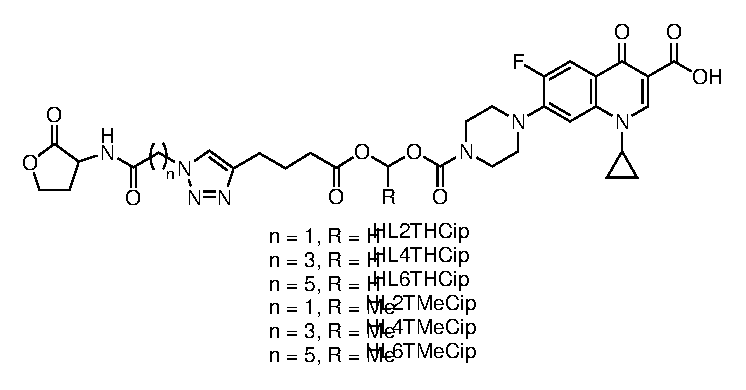
\includegraphics[scale=1]{cleavable_finals}
		\caption{
			The cleavable HSL-Cip triazole conjugates synthesised by Prof. Sotelo.
			\label{fig:cleavable_finals}}
	\end{center}
\end{figure}

In addition, two control compounds \compound{cmpd:BnTHCip} and \compound{cmpd:BnTMeCip} with benzyl head groups were produced by Prof. Sotelo (see \ref{fig:cleavable_controls}). It was hoped that these would show whether the AHL head group is required for activity.

\begin{figure}[H]
	\begin{center}
		\schemeref[BnTHCip]{cmpd:BnTHCip}
		\schemeref[BnTMeCip]{cmpd:BnTMeCip}
		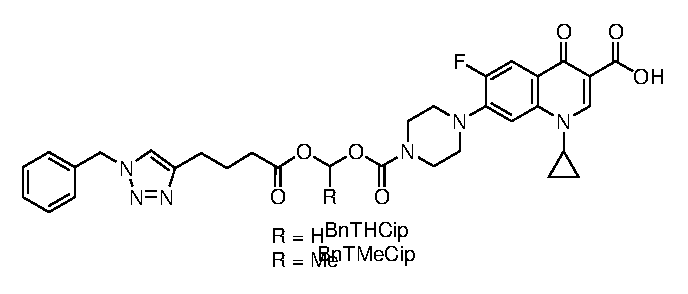
\includegraphics[scale=1]{cleavable_controls}
		\caption{
			The cleavable Bn-Cip triazole conjugates \compound{cmpd:BnTHCip} and \compound{cmpd:BnTMeCip} synthesised by Prof. Sotelo.
			\label{fig:cleavable_controls}}
	\end{center}
\end{figure}



%In the series of ciprofloxacin-AHL containing cleavable linkers synthesised by Prof. Eddy Sotelo, the linker is designed with the hope that the linker will be stable under the extracellular assay conditions, but will be cleaved upon entry into the cell by intracellular esterases. It is hoped that the attached AHLs will facilitate increased uptake into the cells. 
%For the series of compounds with cleavable linkers, in buffered water conditions they are expected to be stable  for '> 3 yrs under optimal conditions', based on the hydrolysis studies of similar compounds in a study by Gogate \cite{Gogate1987}. The optimum conditions for slowest cleavage of these compounds is 4oC and around pH 4.7, whereas LB may reach around pH 8.5\cite{Martin} after 24 hours of bacterial growth and the reaction is run at 30oC, so the degradation rate might be markedly increased under experimental conditions \cite{maths}. 
%In this study the hydrolysis of a secondary amine prodrug is dependent on ester hydrolysis rate in the range 1 =< pH =< 9, therefore the cleavage rate can be tuned by the portion of the molecule between the ester and the triazole, and by the presence of a methyl, hydrogen or other group between the ester and amide\cite{?}. 
%However, initial results in YM64 (a PAO1 mutant lacking efflux pumps) show that the one compound that may show comparable results to ciprofloxacin is a control compound with a benzyl group attached. However, both compounds completely inhibited bacterial growth at all concentrations tested, so it is not clear if the compound is better than ciprofloxacin. Testing in PAO1 should be completed this week; as antibiotics are usually in this wild-type strain the difference between ciprofloxacin and the conjugate should show up without lowering the concentration. 